\section{moeo\-Binary\-Quality\-Indicator$<$ EOFitness $>$ Class Template Reference}
\label{classmoeoBinaryQualityIndicator}\index{moeoBinaryQualityIndicator@{moeoBinaryQualityIndicator}}
Functor Binary quality indicator Binary performance measure to use in the replacement selection process of IBEA (Indicator-Based Evolutionary Algorithm) Of course, EOFitness needs to be an {\bf eo\-Pareto\-Fitness} object.  


{\tt \#include $<$moeo\-Binary\-Quality\-Indicator.h$>$}

Inheritance diagram for moeo\-Binary\-Quality\-Indicator$<$ EOFitness $>$::\begin{figure}[H]
\begin{center}
\leavevmode
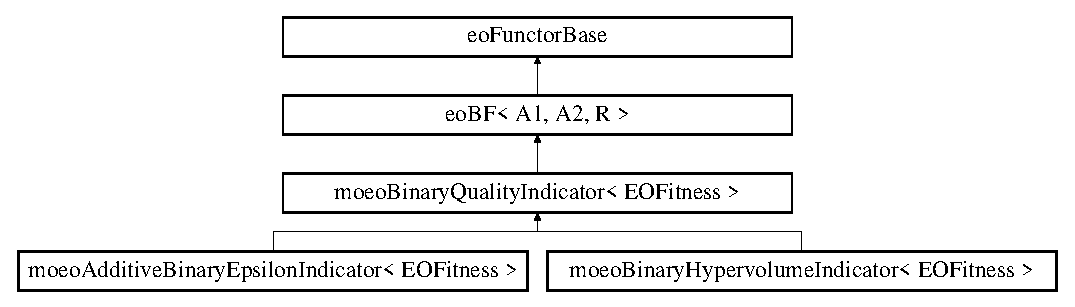
\includegraphics[height=3.67213cm]{classmoeoBinaryQualityIndicator}
\end{center}
\end{figure}
\subsection*{Public Member Functions}
\begin{CompactItemize}
\item 
{\bf moeo\-Binary\-Quality\-Indicator} ()\label{classmoeoBinaryQualityIndicator_a212ae7c8258587a32b158043911cdb6}

\begin{CompactList}\small\item\em constructor \item\end{CompactList}\item 
void {\bf set\-Bounds} (const unsigned \_\-i\-Obj, const double \_\-min, const double \_\-max)
\begin{CompactList}\small\item\em set the bounds for objective \_\-i\-Obj \item\end{CompactList}\end{CompactItemize}
\subsection*{Protected Attributes}
\begin{CompactItemize}
\item 
std::vector$<$ {\bf Range} $>$ {\bf bounds}\label{classmoeoBinaryQualityIndicator_a3bce334c4e74a22c0eb1026592d2f90}

\begin{CompactList}\small\item\em range (min and max double value) for each objective \item\end{CompactList}\end{CompactItemize}
\subsection*{Private Types}
\begin{CompactItemize}
\item 
typedef EOFitness::fitness\_\-traits {\bf traits}\label{classmoeoBinaryQualityIndicator_a23261c88b3ce39b9fed704cad328a76}

\begin{CompactList}\small\item\em fitness traits \item\end{CompactList}\end{CompactItemize}
\subsection*{Classes}
\begin{CompactItemize}
\item 
class {\bf Range}
\begin{CompactList}\small\item\em Private class to represent the bounds. \item\end{CompactList}\end{CompactItemize}


\subsection{Detailed Description}
\subsubsection*{template$<$class EOFitness$>$ class moeo\-Binary\-Quality\-Indicator$<$ EOFitness $>$}

Functor Binary quality indicator Binary performance measure to use in the replacement selection process of IBEA (Indicator-Based Evolutionary Algorithm) Of course, EOFitness needs to be an {\bf eo\-Pareto\-Fitness} object. 



Definition at line 28 of file moeo\-Binary\-Quality\-Indicator.h.

\subsection{Member Function Documentation}
\index{moeoBinaryQualityIndicator@{moeo\-Binary\-Quality\-Indicator}!setBounds@{setBounds}}
\index{setBounds@{setBounds}!moeoBinaryQualityIndicator@{moeo\-Binary\-Quality\-Indicator}}
\subsubsection{\setlength{\rightskip}{0pt plus 5cm}template$<$class EOFitness$>$ void {\bf moeo\-Binary\-Quality\-Indicator}$<$ EOFitness $>$::set\-Bounds (const unsigned {\em \_\-i\-Obj}, const double {\em \_\-min}, const double {\em \_\-max})\hspace{0.3cm}{\tt  [inline]}}\label{classmoeoBinaryQualityIndicator_a08220a55c86a4e0dd1c8977eb625c9f}


set the bounds for objective \_\-i\-Obj 

\begin{Desc}
\item[Parameters:]
\begin{description}
\item[{\em unsigned}]\_\-i\-Obj the index of the objective \item[{\em double}]\_\-min the minimum value \item[{\em double}]\_\-max the maximum value \end{description}
\end{Desc}


Definition at line 51 of file moeo\-Binary\-Quality\-Indicator.h.

Referenced by moeo\-IBEAAvg\-Sorting$<$ EOT, Fitness\-Eval $>$::set\-Bounds(), moeo\-IBEAStoch\-Sorting$<$ EOT, Fitness\-Eval $>$::set\-Bounds(), and moeo\-IBEASorting$<$ EOT, Fitness $>$::set\-Bounds().

The documentation for this class was generated from the following file:\begin{CompactItemize}
\item 
moeo\-Binary\-Quality\-Indicator.h\end{CompactItemize}
